% Copyright 2017 Emilio Rojas
%
% Permission is hereby granted, free of charge, to any person obtaining a copy of
% this software and associated documentation files (the "Software"), to deal in
% the Software without restriction, including without limitation the rights to
% use, copy, modify, merge, publish, distribute, sublicense, and/or sell copies of
% the Software, and to permit persons to whom the Software is furnished to do so,
% subject to the following conditions:
%
% The above copyright notice and this permission notice shall be included in all
% copies or substantial portions of the Software.
%
% THE SOFTWARE IS PROVIDED "AS IS", WITHOUT WARRANTY OF ANY KIND, EXPRESS OR
% IMPLIED, INCLUDING BUT NOT LIMITED TO THE WARRANTIES OF MERCHANTABILITY, FITNESS
% FOR A PARTICULAR PURPOSE AND NONINFRINGEMENT. IN NO EVENT SHALL THE AUTHORS OR
% COPYRIGHT HOLDERS BE LIABLE FOR ANY CLAIM, DAMAGES OR OTHER LIABILITY, WHETHER
% IN AN ACTION OF CONTRACT, TORT OR OTHERWISE, ARISING FROM, OUT OF OR IN
% CONNECTION WITH THE SOFTWARE OR THE USE OR OTHER DEALINGS IN THE SOFTWARE.

\documentclass{article}

% Copyright 2017 Emilio Rojas
%
% Permission is hereby granted, free of charge, to any person obtaining a copy of
% this software and associated documentation files (the "Software"), to deal in
% the Software without restriction, including without limitation the rights to
% use, copy, modify, merge, publish, distribute, sublicense, and/or sell copies of
% the Software, and to permit persons to whom the Software is furnished to do so,
% subject to the following conditions:
%
% The above copyright notice and this permission notice shall be included in all
% copies or substantial portions of the Software.
%
% THE SOFTWARE IS PROVIDED "AS IS", WITHOUT WARRANTY OF ANY KIND, EXPRESS OR
% IMPLIED, INCLUDING BUT NOT LIMITED TO THE WARRANTIES OF MERCHANTABILITY, FITNESS
% FOR A PARTICULAR PURPOSE AND NONINFRINGEMENT. IN NO EVENT SHALL THE AUTHORS OR
% COPYRIGHT HOLDERS BE LIABLE FOR ANY CLAIM, DAMAGES OR OTHER LIABILITY, WHETHER
% IN AN ACTION OF CONTRACT, TORT OR OTHERWISE, ARISING FROM, OUT OF OR IN
% CONNECTION WITH THE SOFTWARE OR THE USE OR OTHER DEALINGS IN THE SOFTWARE.

% Estos son los paquetes que se cargan en todos los documentos, estos paquetes
% están en texlive-full (TODO separar paquetes por seccion de texlive donde
% está el paqeute). De momento se ordenan por longitud del nombre y
% alfabeticamente.

\usepackage{url}
\usepackage{cite}
\usepackage{tikz}

\usepackage{array}
\usepackage{color}
\usepackage{float}

\usepackage{empheq}

\usepackage{amsmath}
\usepackage{apacite}
\usepackage{caption}
\usepackage{gensymb}
\usepackage{siunitx}

\usepackage{amsfonts}
\usepackage{booktabs}
\usepackage{enumitem}
\usepackage{etoolbox}
\usepackage{fancyhdr}
\usepackage{graphicx}
\usepackage{geometry}
\usepackage{hyperref}
\usepackage{mdframed}
\usepackage{multirow}
\usepackage{pdfpages}
\usepackage{pgfplots}
\usepackage{setspace}
\usepackage{textcomp}

\usepackage{adjustbox}
\usepackage{mathtools}

\usepackage{circuitikz}
\usepackage{subcaption}

\usepackage[T1]{fontenc}
\usepackage[spanish]{babel}
\usepackage[utf8]{inputenc}


%%http://tex.stackexchange.com/questions/140567/drawing-karnaughs-maps-in-latex
\usetikzlibrary{matrix,calc}

%isolated term
%#1 - Optional. Space between node and grouping line. Default=0
%#2 - node
%#3 - filling color
\newcommand{\implicantsol}[3][0]{
    \draw[rounded corners=3pt, fill=#3, opacity=0.3] ($(#2.north west)+(135:#1)$) rectangle ($(#2.south east)+(-45:#1)$);
    }


%internal group
%#1 - Optional. Space between node and grouping line. Default=0
%#2 - top left node
%#3 - bottom right node
%#4 - filling color
\newcommand{\implicant}[4][0]{
    \draw[rounded corners=3pt, fill=#4, opacity=0.3] ($(#2.north west)+(135:#1)$) rectangle ($(#3.south east)+(-45:#1)$);
    }

%group lateral borders
%#1 - Optional. Space between node and grouping line. Default=0
%#2 - top left node
%#3 - bottom right node
%#4 - filling color
\newcommand{\implicantcostats}[4][0]{
    \draw[rounded corners=3pt, fill=#4, opacity=0.3] ($(rf.east |- #2.north)+(90:#1)$)-| ($(#2.east)+(0:#1)$) |- ($(rf.east |- #3.south)+(-90:#1)$);
    \draw[rounded corners=3pt, fill=#4, opacity=0.3] ($(cf.west |- #2.north)+(90:#1)$) -| ($(#3.west)+(180:#1)$) |- ($(cf.west |- #3.south)+(-90:#1)$);
}

%group top-bottom borders
%#1 - Optional. Space between node and grouping line. Default=0
%#2 - top left node
%#3 - bottom right node
%#4 - filling color
\newcommand{\implicantdaltbaix}[4][0]{
    \draw[rounded corners=3pt, fill=#4, opacity=0.3] ($(cf.south -| #2.west)+(180:#1)$) |- ($(#2.south)+(-90:#1)$) -| ($(cf.south -| #3.east)+(0:#1)$);
    \draw[rounded corners=3pt, fill=#4, opacity=0.3] ($(rf.north -| #2.west)+(180:#1)$) |- ($(#3.north)+(90:#1)$) -| ($(rf.north -| #3.east)+(0:#1)$);
}

%group corners
%#1 - Optional. Space between node and grouping line. Default=0
%#2 - filling color
\newcommand{\implicantcantons}[2][0]{
    \draw[rounded corners=3pt, opacity=.3] ($(rf.east |- 0.south)+(-90:#1)$) -| ($(0.east |- cf.south)+(0:#1)$);
    \draw[rounded corners=3pt, opacity=.3] ($(rf.east |- 8.north)+(90:#1)$) -| ($(8.east |- rf.north)+(0:#1)$);
    \draw[rounded corners=3pt, opacity=.3] ($(cf.west |- 2.south)+(-90:#1)$) -| ($(2.west |- cf.south)+(180:#1)$);
    \draw[rounded corners=3pt, opacity=.3] ($(cf.west |- 10.north)+(90:#1)$) -| ($(10.west |- rf.north)+(180:#1)$);
    \fill[rounded corners=3pt, fill=#2, opacity=.3] ($(rf.east |- 0.south)+(-90:#1)$) -|  ($(0.east |- cf.south)+(0:#1)$) [sharp corners] ($(rf.east |- 0.south)+(-90:#1)$) |-  ($(0.east |- cf.south)+(0:#1)$) ;
    \fill[rounded corners=3pt, fill=#2, opacity=.3] ($(rf.east |- 8.north)+(90:#1)$) -| ($(8.east |- rf.north)+(0:#1)$) [sharp corners] ($(rf.east |- 8.north)+(90:#1)$) |- ($(8.east |- rf.north)+(0:#1)$) ;
    \fill[rounded corners=3pt, fill=#2, opacity=.3] ($(cf.west |- 2.south)+(-90:#1)$) -| ($(2.west |- cf.south)+(180:#1)$) [sharp corners]($(cf.west |- 2.south)+(-90:#1)$) |- ($(2.west |- cf.south)+(180:#1)$) ;
    \fill[rounded corners=3pt, fill=#2, opacity=.3] ($(cf.west |- 10.north)+(90:#1)$) -| ($(10.west |- rf.north)+(180:#1)$) [sharp corners] ($(cf.west |- 10.north)+(90:#1)$) |- ($(10.west |- rf.north)+(180:#1)$) ;
}

%Empty Karnaugh map 4x4
\newenvironment{Karnaugh}[4]%
{
\begin{tikzpicture}[baseline=(current bounding box.north),scale=0.8]
\draw (0,0) grid (4,4);
\draw (0,4) -- node [pos=0.7,above right,anchor=south west] {#3#4} node [pos=0.7,below left,anchor=north east] {#1#2} ++(135:1);
%
\matrix (mapa) [matrix of nodes,
        column sep={0.8cm,between origins},
        row sep={0.8cm,between origins},
        every node/.style={minimum size=0.3mm},
        anchor=8.center,
        ampersand replacement=\&] at (0.5,0.5)
{
                       \& |(c00)| 00         \& |(c01)| 01         \& |(c11)| 11         \& |(c10)| 10         \& |(cf)| \phantom{00} \\
|(r00)| 00             \& |(0)|  \phantom{0} \& |(1)|  \phantom{0} \& |(3)|  \phantom{0} \& |(2)|  \phantom{0} \&                     \\
|(r01)| 01             \& |(4)|  \phantom{0} \& |(5)|  \phantom{0} \& |(7)|  \phantom{0} \& |(6)|  \phantom{0} \&                     \\
|(r11)| 11             \& |(12)| \phantom{0} \& |(13)| \phantom{0} \& |(15)| \phantom{0} \& |(14)| \phantom{0} \&                     \\
|(r10)| 10             \& |(8)|  \phantom{0} \& |(9)|  \phantom{0} \& |(11)| \phantom{0} \& |(10)| \phantom{0} \&                     \\
|(rf) | \phantom{00}   \&                    \&                    \&                    \&                    \&                     \\
};
}%
{
\end{tikzpicture}
}

%Empty Karnaugh map 2x4
\newenvironment{Karnaughvuit}%
{
\begin{tikzpicture}[baseline=(current bounding box.north),scale=0.8]
\draw (0,0) grid (4,2);
\draw (0,2) -- node [pos=0.7,above right,anchor=south west] {bc} node [pos=0.7,below left,anchor=north east] {a} ++(135:1);
%
\matrix (mapa) [matrix of nodes,
        column sep={0.8cm,between origins},
        row sep={0.8cm,between origins},
        every node/.style={minimum size=0.3mm},
        anchor=4.center,
        ampersand replacement=\&] at (0.5,0.5)
{
                      \& |(c00)| 00         \& |(c01)| 01         \& |(c11)| 11         \& |(c10)| 10         \& |(cf)| \phantom{00} \\
|(r00)| 0             \& |(0)|  \phantom{0} \& |(1)|  \phantom{0} \& |(3)|  \phantom{0} \& |(2)|  \phantom{0} \&                     \\
|(r01)| 1             \& |(4)|  \phantom{0} \& |(5)|  \phantom{0} \& |(7)|  \phantom{0} \& |(6)|  \phantom{0} \&                     \\
|(rf) | \phantom{00}  \&                    \&                    \&                    \&                    \&                     \\
};
}%
{
\end{tikzpicture}
}

%Empty Karnaugh map 2x2
\newenvironment{Karnaughquatre}%
{
\begin{tikzpicture}[baseline=(current bounding box.north),scale=0.8]
\draw (0,0) grid (2,2);
\draw (0,2) -- node [pos=0.7,above right,anchor=south west] {b} node [pos=0.7,below left,anchor=north east] {a} ++(135:1);
%
\matrix (mapa) [matrix of nodes,
        column sep={0.8cm,between origins},
        row sep={0.8cm,between origins},
        every node/.style={minimum size=0.3mm},
        anchor=2.center,
        ampersand replacement=\&] at (0.5,0.5)
{
          \& |(c00)| 0          \& |(c01)| 1  \\
|(r00)| 0 \& |(0)|  \phantom{0} \& |(1)|  \phantom{0} \\
|(r01)| 1 \& |(2)|  \phantom{0} \& |(3)|  \phantom{0} \\
};
}%
{
\end{tikzpicture}
}

%Defines 8 or 16 values (0,1,X)
\newcommand{\contingut}[1]{%
\foreach \x [count=\xi from 0]  in {#1}
     \path (\xi) node {\x};
}

%Places 1 in listed positions
\newcommand{\minterms}[1]{%
    \foreach \x in {#1}
        \path (\x) node {1};
}

%Places 0 in listed positions
\newcommand{\maxterms}[1]{%
    \foreach \x in {#1}
        \path (\x) node {0};
}

%Places X in listed positions
\newcommand{\indeterminats}[1]{%
    \foreach \x in {#1}
        \path (\x) node {X};
}

% Copyright 2017 Emilio Rojas
%
% Permission is hereby granted, free of charge, to any person obtaining a copy of
% this software and associated documentation files (the "Software"), to deal in
% the Software without restriction, including without limitation the rights to
% use, copy, modify, merge, publish, distribute, sublicense, and/or sell copies of
% the Software, and to permit persons to whom the Software is furnished to do so,
% subject to the following conditions:
%
% The above copyright notice and this permission notice shall be included in all
% copies or substantial portions of the Software.
%
% THE SOFTWARE IS PROVIDED "AS IS", WITHOUT WARRANTY OF ANY KIND, EXPRESS OR
% IMPLIED, INCLUDING BUT NOT LIMITED TO THE WARRANTIES OF MERCHANTABILITY, FITNESS
% FOR A PARTICULAR PURPOSE AND NONINFRINGEMENT. IN NO EVENT SHALL THE AUTHORS OR
% COPYRIGHT HOLDERS BE LIABLE FOR ANY CLAIM, DAMAGES OR OTHER LIABILITY, WHETHER
% IN AN ACTION OF CONTRACT, TORT OR OTHERWISE, ARISING FROM, OUT OF OR IN
% CONNECTION WITH THE SOFTWARE OR THE USE OR OTHER DEALINGS IN THE SOFTWARE.

% allows to use < and > on tikz pictures when babel set to spanish
% http://tex.stackexchange.com/questions/166772/problem-with-babel-and-tikz-using-draw
\usetikzlibrary{babel}
\usetikzlibrary{positioning}
\usetikzlibrary{quotes, angles}

\pgfplotsset{compat=1.13}

\setlength
  {\columnsep}
  {1cm}

\patchcmd
  {\chapter}
  {\thispagestyle{plain}}
  {\thispagestyle{fancy}}
  {}
  {}

\geometry
  {
    a4paper,
    left=25.4mm,
    right=25.4mm,
    top=25.4mm,
    bottom=25.4mm,
    heightrounded,
  }

\sisetup{output-exponent-marker=\textsc{e}}
\setlength{\jot}{10pt}

% FANCY SETTINGS
\pagestyle{fancy}
\fancyhf{}
\lhead{Circuitos Digitales I}
\rfoot{\thepage}
\setlength{\headheight}{20pt}

% ZENER
\makeatletter
\pgfcircdeclarebipole{}{
  \ctikzvalof{bipoles/diode/height}
}{fullzzdiode}{
  \ctikzvalof{bipoles/diode/height}
}{
  \ctikzvalof{bipoles/diode/width}
}{

  \pgfsetlinewidth{\pgfkeysvalueof{/tikz/circuitikz/bipoles/thickness}\pgfstartlinewidth}

  \pgfscope
    \pgftransformxshift{\pgf@circ@res@left}
    \pgfpathmoveto{\pgfpoint{\pgf@circ@res@right-\pgf@circ@res@left}{0pt}}
    \pgfpathlineto{\pgfpoint{0pt}{\pgf@circ@res@up}}
    \pgfpathlineto{\pgfpoint{0pt}{\pgf@circ@res@down}}
    \pgfpathlineto{\pgfpoint{\pgf@circ@res@right-\pgf@circ@res@left}{0pt}}
    \pgfusepath{draw,fill}
    \pgfpathmoveto{
      \pgfpoint{
        \pgf@circ@res@right-1.8\pgf@circ@res@left
      }{
        \pgf@circ@res@down-0.5\pgf@circ@res@up
      }
    }
    \pgfpathlineto{
      \pgfpoint{
        \pgf@circ@res@right-\pgf@circ@res@left
      }{
        \pgf@circ@res@down
      }
    }
    \pgfpathlineto{
      \pgfpoint{
        \pgf@circ@res@right-\pgf@circ@res@left
      }{
        \pgf@circ@res@up
      }
    }
    \pgfpathlineto{
      \pgfpoint{
        \pgf@circ@res@right-0.2\pgf@circ@res@left
      }{
        \pgf@circ@res@up-0.5\pgf@circ@res@down
      }
    }
    \pgfusepath{draw}
  \endpgfscope
}
\def\pgf@circ@fullzzdiode@path#1{\pgf@circ@bipole@path{fullzzdiode}{#1}}
\tikzset{full Zzener diode/.style = {\circuitikzbasekey, /tikz/to path=\pgf@circ@fullzzdiode@path}}
\tikzset{zzD*/.style = {full Zzener diode}}
\makeatother

% Copyright 2017 Emilio Rojas
%
% Permission is hereby granted, free of charge, to any person obtaining a copy of
% this software and associated documentation files (the "Software"), to deal in
% the Software without restriction, including without limitation the rights to
% use, copy, modify, merge, publish, distribute, sublicense, and/or sell copies of
% the Software, and to permit persons to whom the Software is furnished to do so,
% subject to the following conditions:
%
% The above copyright notice and this permission notice shall be included in all
% copies or substantial portions of the Software.
%
% THE SOFTWARE IS PROVIDED "AS IS", WITHOUT WARRANTY OF ANY KIND, EXPRESS OR
% IMPLIED, INCLUDING BUT NOT LIMITED TO THE WARRANTIES OF MERCHANTABILITY, FITNESS
% FOR A PARTICULAR PURPOSE AND NONINFRINGEMENT. IN NO EVENT SHALL THE AUTHORS OR
% COPYRIGHT HOLDERS BE LIABLE FOR ANY CLAIM, DAMAGES OR OTHER LIABILITY, WHETHER
% IN AN ACTION OF CONTRACT, TORT OR OTHERWISE, ARISING FROM, OUT OF OR IN
% CONNECTION WITH THE SOFTWARE OR THE USE OR OTHER DEALINGS IN THE SOFTWARE.

% Unnumbered section added to toc
% 1: The section's name.
\newcommand{\usection}[1]
{
  \section*{#1}
  \addcontentsline{toc}{section}{#1}
}

% Unnumbered subsection added to toc
% 1: The subsection's name.
\newcommand{\usubsection}[1]
{
  \subsection*{#1}
  \addcontentsline{toc}{subsection}{#1}
}

% Unnumbered subsubsection added to toc
% 1: The subsubsection's name.
\newcommand{\usubsubsection}[1]
{
  \subsubsection*{#1}
  \addcontentsline{toc}{subsubsection}{#1}
}

% Uncut table rules
\makeatletter
\newlength\mylena
\newlength\mylenb
\newcommand\mystrut[1][2]{%
    \setlength\mylena{#1\ht\@arstrutbox}%
    \setlength\mylenb{#1\dp\@arstrutbox}%
    \rule[\mylenb]{0pt}{\mylena}}
\makeatother

% Circuitikz equal
\newcommand*{\equal}{=}

% Adds a title page to the document
% 1: The document's name
% 2: The document's owner's name
% 3: The document's owner's id
% 4: The document's date

% \portada{Homework}{John Doe}{123456}{\today}
\newcommand{\portada}[4]
{
  \begin{titlepage}
    \vspace*{\fill}
    \begin{center}

      \textsc{\Large Universidad de Costa Rica}\\
      [0.25in]

      \textsc{\Large Escuela de Ingeniería Eléctrica}\\
      [0.55in]

      \textsc{\Large Circuitos Digitales I - IE0323}\\
      [0.25in]

      \textsc{\huge \bfseries {#1}}\\
      [0.5in]

      \textsc{\large {#2}}\\
      \textsc{\large {#3}}\\
      [0.5in]

      \textsc{\large {#4}}
    \end{center}
    \vspace*{\fill}
  \end{titlepage}
}


\begin{document}

\pagenumbering{gobble}

\portada
{Tarea \#5 {\large y} \#6}
{Emilio Javier Rojas Álvarez}
{B15680}
{\today}

\usection{Introducción}
Se construye un circuito que maneja un sistema semáforo de paso peatonal y el
respectivo vehicular. Para esto se utiliza una máquina de estados con 8 estados,
4 de los cuales son para cargar un tiempo en un contador, y los otros 4 son para
esperar que ese tiempo transcurra. Adicionalmente se pudo haber tomado en cuenta
una serie de estados que tomara en cuenta si el tiempo habia transcurrido, sin
embargo se decidió utilizar una memoria externa para saber si el tiempo habia
transcurrido, similar a la memoria de la solicitud de paso, esta solución tiene
la desventaja de que, sin lógica adicional, no permite deshabilitar el contador
cuando no se necesite, por lo que este está contando en todo momento.

El circuito creado se muestra en la figura 1, y cuenta con 5 bloques. 2 memorias
de estados para SP(solicitud de paso), y ZERO(indica si el contador ha marcado 0),
la máquina de estados, compuesta por 3 flip flops JK, lógica de entrada y lógica
de salida, un decodificador de salidas para indicar cuales luces de los semáforos
deben encenderse, y por último un módulo de tiempos que es el encargado de
contar y enviar las señales a las pantallas de 7 segmentos.

\begin{figure}[H]
  \centering
  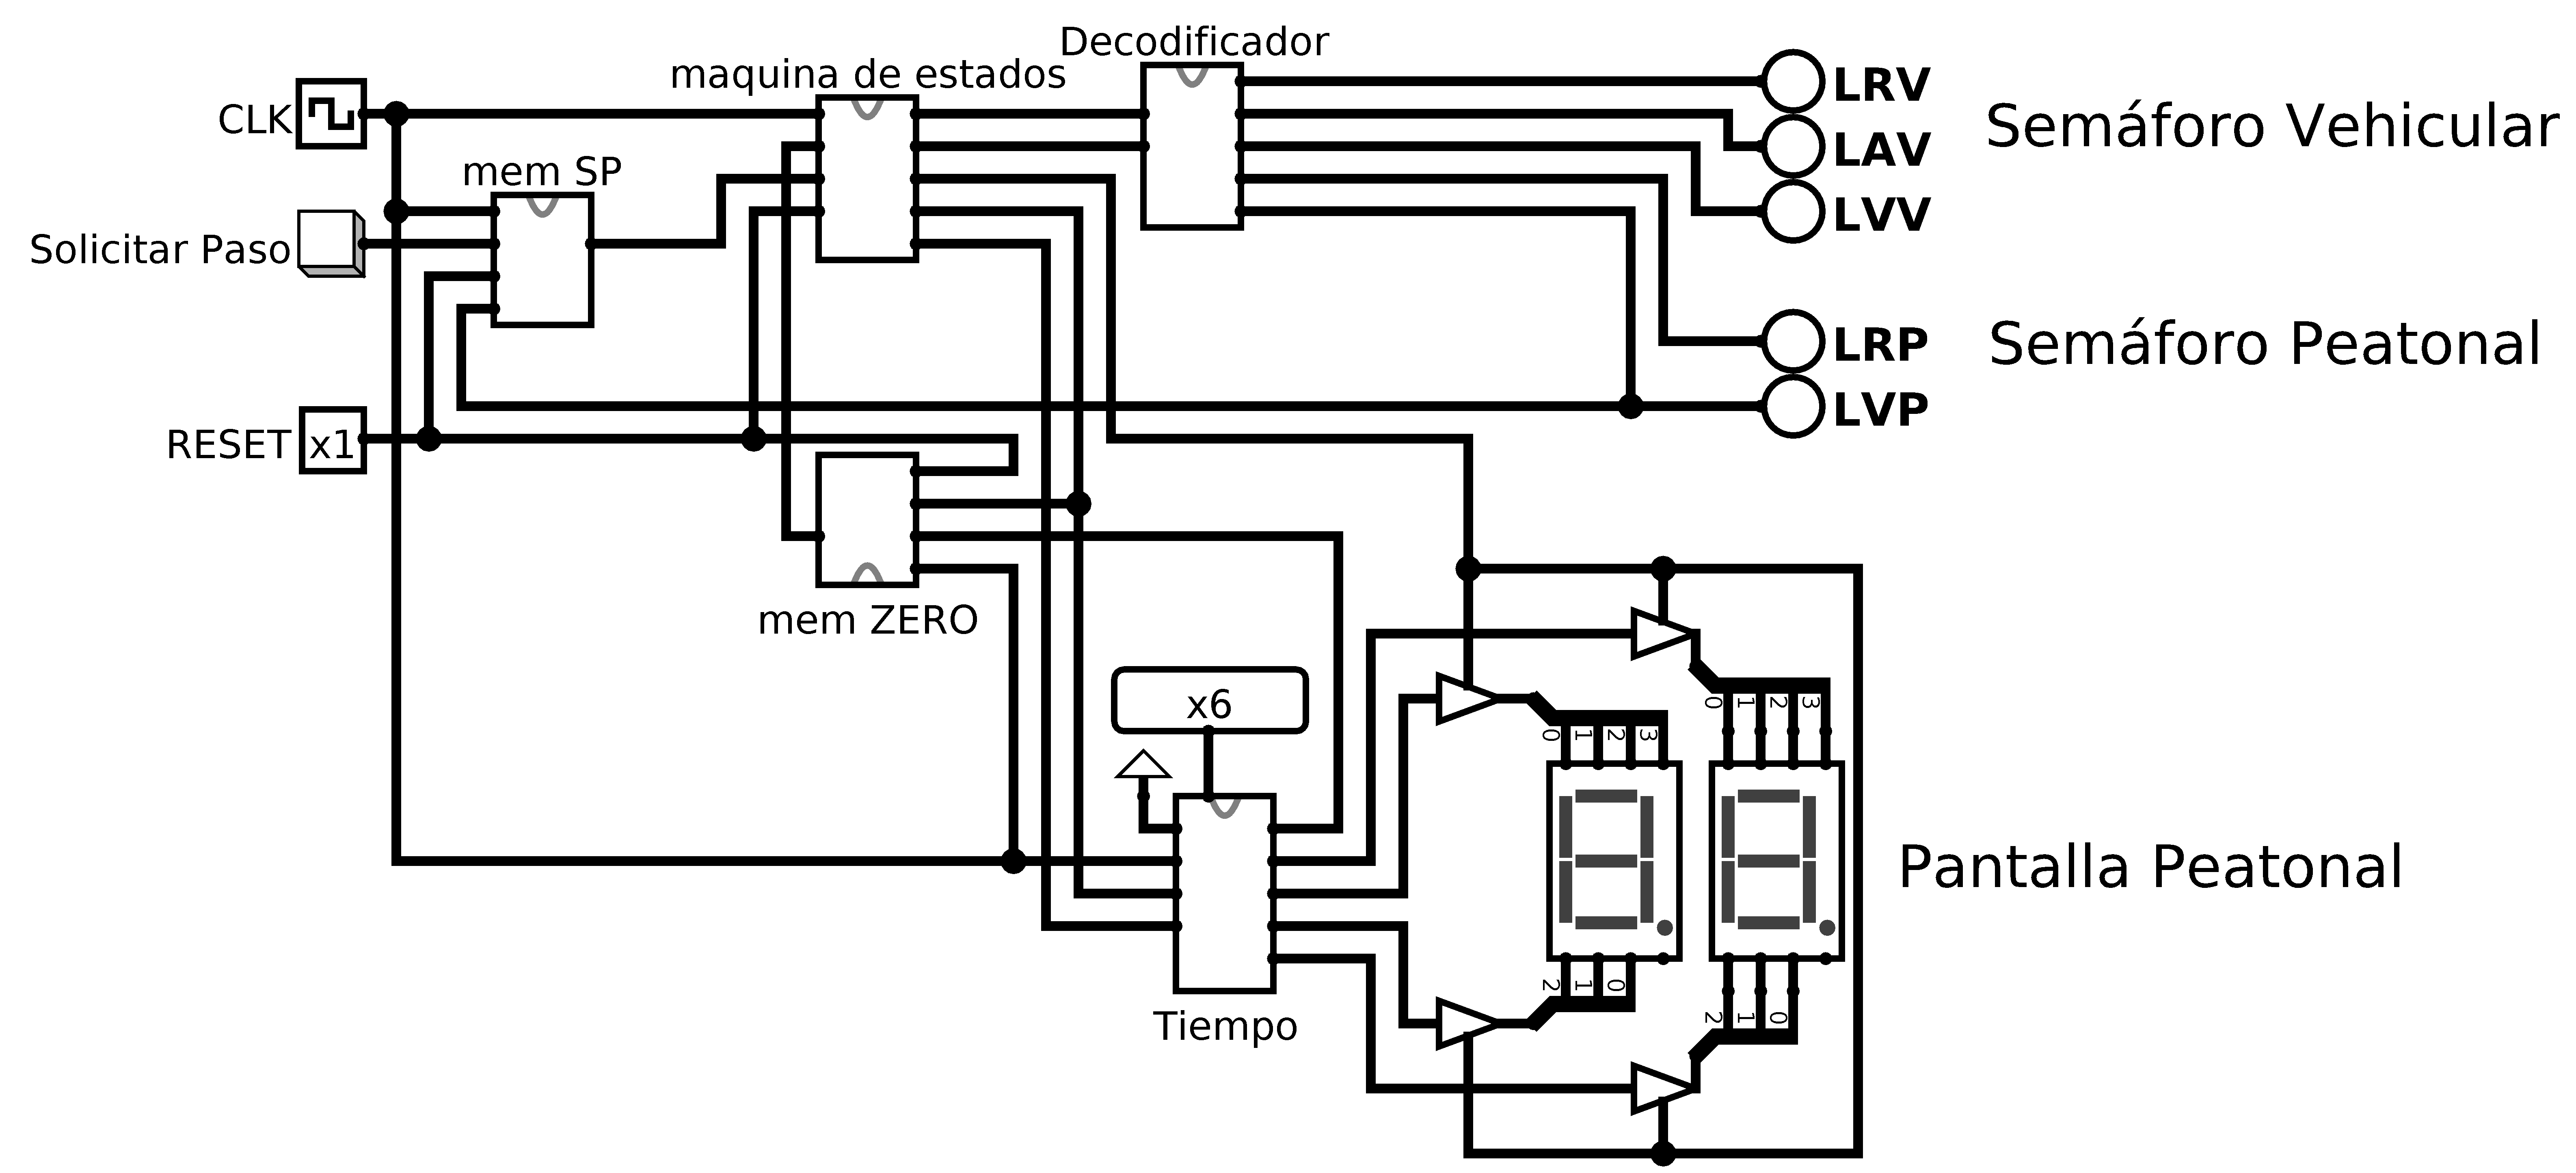
\includegraphics[width=0.75\textwidth]{circuito/main.png}
  \caption{Circuito para el sistema solicitado.}
\end{figure}

\usection{Descripción del Algoritmo utilizado}

% Copyright 2017 Emilio Rojas
%
% Permission is hereby granted, free of charge, to any person obtaining a copy of
% this software and associated documentation files (the "Software"), to deal in
% the Software without restriction, including without limitation the rights to
% use, copy, modify, merge, publish, distribute, sublicense, and/or sell copies of
% the Software, and to permit persons to whom the Software is furnished to do so,
% subject to the following conditions:
%
% The above copyright notice and this permission notice shall be included in all
% copies or substantial portions of the Software.
%
% THE SOFTWARE IS PROVIDED "AS IS", WITHOUT WARRANTY OF ANY KIND, EXPRESS OR
% IMPLIED, INCLUDING BUT NOT LIMITED TO THE WARRANTIES OF MERCHANTABILITY, FITNESS
% FOR A PARTICULAR PURPOSE AND NONINFRINGEMENT. IN NO EVENT SHALL THE AUTHORS OR
% COPYRIGHT HOLDERS BE LIABLE FOR ANY CLAIM, DAMAGES OR OTHER LIABILITY, WHETHER
% IN AN ACTION OF CONTRACT, TORT OR OTHERWISE, ARISING FROM, OUT OF OR IN
% CONNECTION WITH THE SOFTWARE OR THE USE OR OTHER DEALINGS IN THE SOFTWARE.

\usubsection{Estados}
Se definen 8 estados con los bits $X$, $Y$ y $Z$. $X$ representa a $S_1$ y $Y$ a $S_0$.
\begin{enumerate}[label*=\textbf{\alph*)}]
  \item $X=0$, $Y=0$, $Z=0$: Carga tiempo mínimo de paso vehicular.
  \item $X=0$, $Y=0$, $Z=1$: Espera tiempo mínimo de paso vehicular y solicitud de paso.
  \item $X=0$, $Y=1$, $Z=0$: Carga de tiempo de paso restringido(luz amarilla vehicular).
  \item $X=0$, $Y=1$, $Z=1$: Espera tiempo de paso restringido.
  \item $X=1$, $Y=0$, $Z=0$: Carga de tiempo de paso peatonal.
  \item $X=1$, $Y=0$, $Z=1$: Espera tiempo de paso peatonal.
  \item $X=1$, $Y=1$, $Z=0$: Carga de tiempo de banda de seguridad(luz roja vehicular y luz roja peatonal).
  \item $X=1$, $Y=1$, $Z=1$: Espera tiempo de banda de seguridad.
\end{enumerate}


El algoritmo utilizado es bastante sencillo, principalmente porque el usuario(el peatón)
solo tiene una manera de interactuar con el sistema, solicitando el paso, esto
corresponde al estado \textbf{b}. El sistma comienza en el estado \textbf{a}, donde
carga 40 segundos(mínimo) para el paso vehicular, y pasa al estado \textbf{b} que
espera la señal de ZERO(han transcurrido los 40 segundos) y la solicitud de paso,
una vez cumplidas estas condiciones se pasa al estado \textbf{c}, que carga 10
segundos para el paso restringido(esto es cuando la luz amarilla vehicular está
encendida y la luz peatonal se mantien en rojo), y se procede a esperar esos 10
segundos en el estado \textbf{d}, y se sigue inmediatamente en el estado \textbf{e},
se carga 40 segundos para el paso peatonal, y se espera estos 40 segundos en el
estado \textbf{f}, donde también se encienden las pantallas de 7 segmentos.
Por último, se tienen los estados \textbf{g} y \textbf{h}, el primero carga 10
segundos en los cuales los 2 semáforos están en rojo, y el segundo se encarga de
esperar que trancurra dicho tiempo. Una vez cumplido el tiempo se regresa al estado
\textbf{a}.

\usection{Diagrama ASM}
Se muestra el diagrama ASM, se omiten las salidas $S_1$, $S_0$ puesto que están
dadas por el código del estado.
\usetikzlibrary{arrows, arrows.meta, shapes}
\begin{figure}[H]
  \centering
  \tikz[scale=0.9]{
    \draw
    (0, 0) node {a} circle (.5)
    ++(-1.5, -.5) rectangle ++(3, -1) ++(-1.5, .5) node (ae1) {LOAD}
    ;
    \draw[->]
    (ae1) ++(0, -.5) -- ++(0, -.5) node (a1) {}
    ;
    \draw
    (a1) ++(0, -.5) node {b} circle (.5)
    ++(0, -.5) -- ++(2, -.5) -- ++(-2, -.5) node (q11) {} -- ++(-2, .5) node (q10) {} -- ++(2, .5)
    ++(0, -.5) node {ZERO$\cdot$SP'}
    ++(-2, .5) node (ae2) {}
    ;
    \draw[->]
    (q10) node [above left] {0} -- ++(0, 1) -- ++(1.5, 0)
    ;
    \draw[->]
    (q11) node [below left] {1} -- ++(0, -.5) node (a2) {}
    ;


    \draw
    (a2) ++(0, -.5) node {c} circle (.5)
    ++(-1.5, -.5) rectangle ++(3, -1) ++(-1.5, .5) node (ae3) {LOAD, TS}
    ;
    \draw[->]
    (ae3) ++(0, -.5) -- ++(0, -.5) node (a3) {};
    \draw
    (a3) ++(0, -.5) node {d} circle (.5)
    ++(0, -.5) -- ++(2, -.5) -- ++(-2, -.5) node (q21) {} -- ++(-2, .5) node (q20) {} -- ++(2, .5)
    ++(0, -.5) node {ZERO}
    ++(-2, .5) node (ae4) {}
    ;
    \draw[->]
    (q20) node [above left] {0} -- ++(0, 1) -- ++(1.5, 0)
    ;
    \draw[->]
    (q21) node [below left] {1} -- ++(0, -.5) node (a4) {}
    ;

    \draw
    (a4) ++(0, -.5) node {e} circle (.5)
    ++(-1.5, -.5) rectangle ++(3, -1) ++(-1.5, .5) node (ae5) {LOAD}
    ;
    \draw[->]
    (ae5) ++(0, -.5) -- ++(0, -.5) node (a5) {};

    \draw
    (a5) ++(0, -.5) node {f} circle (.5)
    ++(-1.5, -.5) rectangle ++(3, -1) ++(-1.5, .5) node {SE}
    ++(0, -.5) -- ++(2, -.5) -- ++(-2, -.5) node (q31) {} -- ++(-2, .5) node (q30) {} -- ++(2, .5)
    ++(0, -.5) node {ZERO}
    ++(-2, .5) node (ae6) {}
    ;
    \draw[->]
    (q30) node [above left] {0} -- ++(0, 2) -- ++(1.5, 0)
    ;
    \draw[->]
    (q31) node [below left] {1} -- ++(0, -.5) node (a6) {}
    ;

    \draw
    (a6) ++(0, -.5) node {g} circle (.5)
    ++(-1.5, -.5) rectangle ++(3, -1) ++(-1.5, .5) node (ae7) {LOAD, TS}
    ;
    \draw[->]
    (ae7) ++(0, -.5) -- ++(0, -.5) node (a7) {};
    \draw
    (a7) ++(0, -.5) node {h} circle (.5)
    ++(0, -.5) -- ++(2, -.5) -- ++(-2, -.5) node (q41) {} -- ++(-2, .5) node (q40) {} -- ++(2, .5)
    ++(0, -.5) node {ZERO}
    ++(-2, .5) node (ae8) {}
    ;
    \draw[->]
    (q40) node [above left] {0} -- ++(0, 1) -- ++(1.5, 0)
    ;
    \draw[->]
    (q41) node [below left] {1} -- ++(0, -.5) -- ++(2.5, 0) -- ++(0, 20.5) -- ++(-2, 0)
    ;
  }
\end{figure}


\end{document}
